\chapter{New ``Where Am I" Algorithm}
\label{app:A}

This appendix includes a disscussion of the new particle location and material update (``where am I")
algorithm in the WARP code. The discussion is included here as an appendix because this algorithm was 
updated after the original presentation corresponding to the master's degree and this report.

The original algorithm, discussed in Section \ref{sec:rt}, was found to produce incorrect results when 
testing the experimental material and geometry configurations discussed in Section \ref{sec:exp}.
Because of this, the particle location update algorithm was modified to be able to
correctly handle such configurations in addition to the ones originally tested.

WARP now uses ``cell sense" in its ray tracing implementation to determine in which cell and material a
neutron is located. Cell sense is positive if a neutron is outside of a cell and negative if a neutron is
inside of a cell; it is the product of the surface senses of the cell's constituent planes. Figure 
\ref{whereaminew} shows an illustration of the process.

\begin{figure}[h!]
\centering
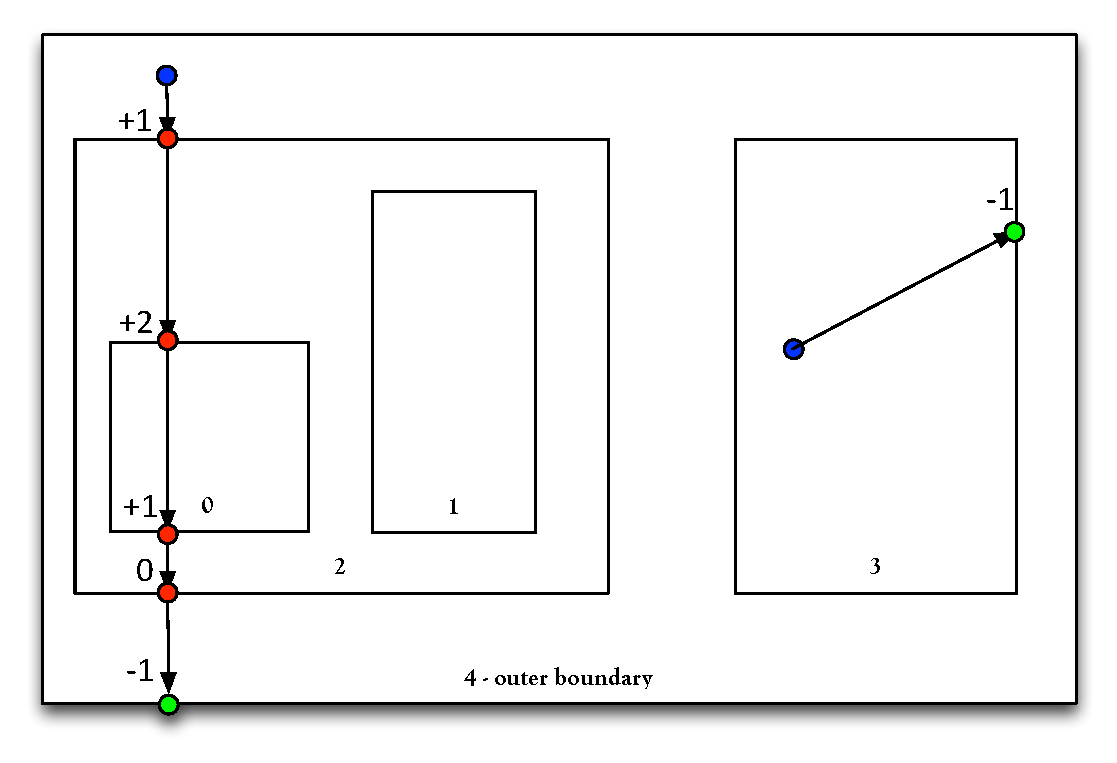
\includegraphics[width=0.9\textwidth]{img/whereami-new.pdf}
\caption{The new, improved point-in-polygon ``where am I" algorithm. \label{whereaminew}}
\end{figure}

In WARP, the surface normal vectors always point outward and the signs of the normals encountered along a
trace are summed in the tracing process. When the sum becomes negative, the trace is stopped, and the 
last intersected cell (and its corresponding material) is the one in which the neutron is located.

Previously, a list of cell numbers was stored for each cell surface intersection that occurred along the
trace with the double entries removed to make a nested list of the cell(s) in which a neutron was 
located. In the new algorithm, cell sense is calculated on the fly as the query ray traverses the
configuration geometry, allowing the trace to stop as soon as the cumulative sense becomes negative. This
is possible because WARP requires that all geometry surfaces be closed. Additionally, compared to the
prior scheme of storing and operating on a list of integers, this new method only requires a single 
integer to be stored and operated on.
